\documentclass[a4paper,12pt,twosided]{report}
\usepackage[portuguese]{babel}
\usepackage[T1]{fontenc}
\usepackage[margin=3cm]{geometry}
\usepackage{newtxtext,newtxmath,graphicx,hyperref}
\hypersetup{
  bookmarksopen=true,
  colorlinks=true,
  linkcolor=blue,
  citecolor=magenta,
  urlcolor=green,
  pdftitle={Leis de Newton},
  pdfauthor={Jaime E. Villate},
  pdfsubject={Mecânica},
  pdfkeywords={dinâmica, mecânica, Newton, atrito},
}
\urlstyle{same}
\setlength{\parindent}{0pt}
\setlength{\parskip}{0.7em}
\pagestyle{headings}

\begin{document}

\begin{titlepage}
\begin{center}
\vspace*{4cm}
{\bfseries\huge Mecânica clássica}
\vfill
{\slshape\Large Jaime Villate}\\
{\large Faculdade de Engenharia da Universidade do Porto}
\vfill
Porto, Portugal\\
2 de dezembro de 2021
\vfill
\end{center}
\end{titlepage}

\tableofcontents
\listoffigures
\listoftables

\chapter{Leis de Newton}

\section{Introdução}

As três leis de Newton são a base da mecânica clássica, que permite
estudar desde o movimento dos objetos à nossa volta, até o movimento
dos planetas, estrelas e outros objetos distantes.  As 3 leis foram
enunciadas de forma clara numa única página do livro escrito por
Newton em 1687~\cite{Newton}.

\begin{table}
  \centering
  \begin{tabular}{|l|l|}
    \hline
    $m$ & Massa.\\
    \hline
    $\vec{v}$ & Velocidade.\\
    \hline
    $\vec{p}$ & Quantidade de movimento.\\
    \hline
    $\vec{F}$ & Força.\\
    \hline
  \end{tabular}
  \caption[Símbolos]{Símbolos usados para as grandezas físicas.}
  \label{tab:simbolos}
\end{table}
\section{Lei da inércia}

A primeira lei de Newton, denominada lei da inércia, foi enunciada por
Newton no seu livro assim:

\begin{quotation}
\noindent\textbf{LEI I.}\\
\emph{``Todo corpo mantém o seu estado de repouso\index{repouso} ou de
movimento uniforme segundo uma linha reta, se não for compelido a mudar o
seu estado por forças nele impressas}.

Os projéteis continuam no seu movimento,\index{movimento!uniforme} a menos
que sejam retardados pela resistência do ar ou impelidos para baixo pela
força da gravidade. Um pião, cujas partes, pela sua coesão, são
continuamente desviadas dos seus movimentos retilíneos, não cessa de
rodar se não for retardado pelo ar. Os corpos maiores --- planetas e
cometas --- encontrando menos resistência nos espaços livres, continuam
os seus movimentos, retilíneos ou circulares, por tempo muito maior.''
\end{quotation}

\section{Força e aceleração}

A segunda lei de Newton pode ser considerada a definição do vetor
associado a uma força, medido em função do efeito que produz sobre os
corpos em que atua. O texto original do livro de Newton é:

\begin{quotation}
\noindent\textbf{LEI II.}\\
\emph{``A mudança na quantidade de movimento é proporcional à força
motora impressa e faz-se na direção da linha reta segundo a qual a força
motora é aplicada}.

Se uma força gera uma quantidade de movimento, uma força dupla gerará
uma quantidade de movimento dupla, uma força tripla gerará uma quantidade
de movimento tripla, quer a força seja impressa de uma vez e
imediatamente, quer seja impressa gradual e sucessivamente. E se o corpo
já então se movia, a nova quantidade de movimento (sempre dirigida na
direção da força atuante) é adicionada ou subtraída à quantidade de
movimento inicial, conforme sejam concordantes ou opostas uma da outra; ou
juntas obliquamente de forma a produzir uma nova quantidade de movimento
composta pela determinação das duas.''
\end{quotation}

Uma das oito definições que antecedem o enunciado das três leis no
livro de Newton é a definição de \textbf{quantidade de movimento}, que
é o produto da massa e a velocidade de um corpo.\footnote{A quantidade de
movimento também costuma chamar-se momento linear.} A explicação a
seguir à segunda lei, sobre como somar a quantidade de movimento
devida a uma força, com a quantidade de movimento que o objeto já
tinha, corresponde à nossa definição atual de adição de vetores. Como
tal, na notação usada atualmente a quantidade de movimento definida
por Newton é um vetor $\vec{p}$, igual ao produto da massa do objeto
vezes a sua velocidade\footnote{Usaremos setas por cima das variáveis que
  representam vetores.}
\begin{equation}
\vec{p} = m\,\vec{v}
\end{equation}

A ``mudança da quantidade de movimento'', referida na segunda lei, é a
quantidade de movimento final, $\vec{p}_2$, menos a quantidade de movimento
inicial, $\vec{p}_1$ e, como é dito no enunciado da lei, essa mudança de
quantidade de movimento é um vetor com a mesma direção e sentido da
força que a produz. A frase ``quer a força seja impressa de uma vez e
imediatamente, quer seja impressa gradual e sucessivamente'' significa que
a mudança na quantidade de movimento é igual ao integral da força
durante o intervalo de tempo em que atua. Como tal, a expressão
matemática da segunda lei de Newton é:
\begin{equation}
\label{lei1}
 \int_{t_1}^{t_2}\vec{F}\,\mathrm{d}\,t = \vec{p}_2 - \vec{p}_1
\end{equation}

A força $\vec{F}$ na equação \ref{lei1} deverá ser interpretada como a
força resultante que atua sobre o objeto, ou seja, a
\href{https://villate.org/dinamica/cinematica_vetorial.html#sec-2.3}{soma
  vetorial} de todas as forças aplicadas sobre o objeto

O integral da força resultante, no lado esquerdo da equação
\ref{lei1}, dá como resultado um vetor $\vec{I}$ chamado
\textbf{impulso}. Como tal, se uma força atua durante um intervalo de
tempo [$t _{1}$, $t _{2}$] sobre um corpo com quantidade de movimento
inicial $\vec{p}_1$, a sua quantidade de movimento no instante
$t _{2}$ será $\vec{p} _{2}$ = $\vec{p} _{1}$ + $\vec{I}$.

A equação \ref{lei1} pode ser escrita de forma diferencial, ou seja,
\begin{equation}
\vec{F} = \frac{\mathrm{d}\,\vec{p}}{\mathrm{d}\,t}
\end{equation}

E quando a massa do corpo permanece constante, substituindo $\vec{p}$ por
$m\,\vec{v}$ conduz à seguinte equação
\begin{equation}
\vec{F} = m\,\vec{a}
\end{equation}
onde $\vec{a}$ é a aceleração do corpo, igual à derivada da sua
velocidade em ordem ao tempo. Esta é a forma mais habitual de escrever
a segunda lei de Newton.

\section{Lei de ação e reação}

A terceira lei, conhecida como \textbf{lei de ação e reação}, é:

\begin{figure}[!b]
\centering
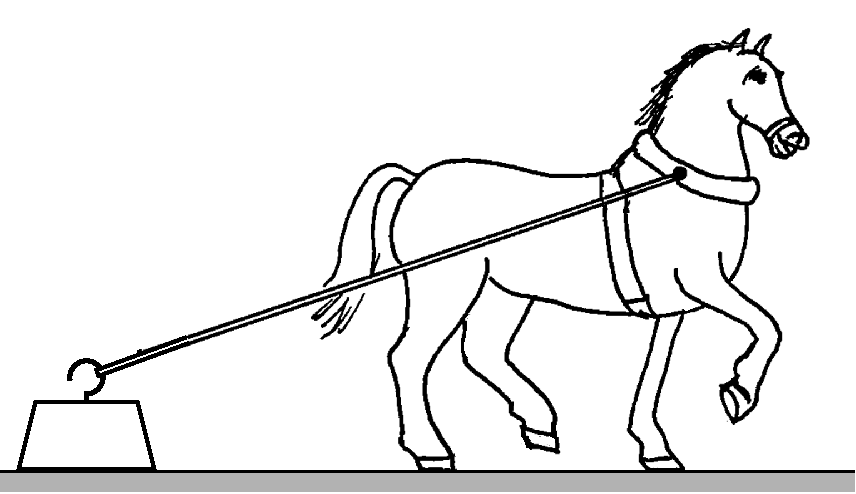
\includegraphics[width=0.8\textwidth]{cavalo.pdf}
\caption{Cavalo a arrastar um bloco.}
\label{fig:cavalo}
\end{figure}

\begin{quotation}
\noindent\textbf{LEI III.}\\
``\emph{A toda a ação opõe sempre uma igual
reação\index{reacao@reação}.  Isto é, as ações mútuas de dois
corpos um sobre o outro são sempre iguais e opostas}.

Aquilo que puxa ou comprime outra coisa é puxado ou comprimido da mesma
maneira por essa coisa. Se premir uma pedra com um dedo, o dedo é
igualmente premido pela pedra. Se um cavalo puxar uma pedra por meio de uma
corda, o cavalo será puxado para trás igualmente em direção à pedra.
Pois a corda esticada tanto puxa o cavalo para a pedra como puxa a pedra
para o cavalo, tanto dificulta a progressão do cavalo como favorece a
progressão da pedra. Se um corpo bater noutro e pela sua força lhe mudar
a quantidade de movimento, sofrerá igual mudança na sua quantidade de
movimento, em sentido oposto. As mudanças feitas por estas ações são
iguais, não nas velocidades, mas nas quantidades de movimento dos corpos.
Isto, suposto que os corpos não são retidos por outros impedimentos.
Portanto, se as quantidades de movimento são mudadas de igual, as
mudanças de velocidades em sentido contrário são inversamente
proporcionais às massas dos corpos.''
\end{quotation}

No exemplo dado por Newton, em que um cavalo arrasta um bloco pesado
por meio de uma corda (figura \ref{fig:cavalo}). O cavalo exerce uma
força para a direita sobre o bloco, através da corda, e o bloco exerce
uma força igual e oposta sobre o cavalo, para a esquerda.  opostos.

\chapter{Forças}

\section{Peso}
No vácuo todos os objetos em queda livre são acelerados com a
\textbf{aceleração da gravidade}, que na superfície terrestre tem um
valor $g$ constante~\cite{French}.

Como tal, de acordo com a segunda lei de Newton o peso de qualquer
objeto (força gravítica exercida pela Terra) é diretamente
proporcional à sua massa:
\begin{equation}
  \vec{P} = m\,\vec{g}
\end{equation}
em que $\vec{g}$ é um vetor constante na direção vertical, com sentido
de cima para baixo e módulo igual à aceleração da gravidade, $g$, que
é aproximadamente igual a 9.8~m/s$^{2}$.

\section{Reação normal e força de atrito}

A força de contacto entre as superfícies de dois objeto podem apontar
em qualquer direção, mas o sentido é sempre no sentido em que as duas
superfícies tendem a se afastar.  É habitual separar essas forças de
contacto em duas componentes, uma componente perpendicular às
superfícies em contacto, chamada \textbf{reação normal} e outra
componente tangente às superfícies, denominada \textbf{força de
  atrito}.

A força de contacto entre superfícies é realmente uma força
distribuída em vários pontos da superfície. A resultante de todas
essas forças será representada num ponto da superfície, separando as
componentes normal e tangencial (figura \ref{fig:contacto}). A reação
normal, $R_\mathrm{n}$ terá sempre o sentido que faz separar os dois
corpos em contacto. A força de atrito, $\vec{F}_\mathrm{a}$, pode ter
qualquer um dos dois sentidos na direção tangencial.

\begin{figure}[hbt]
\centering
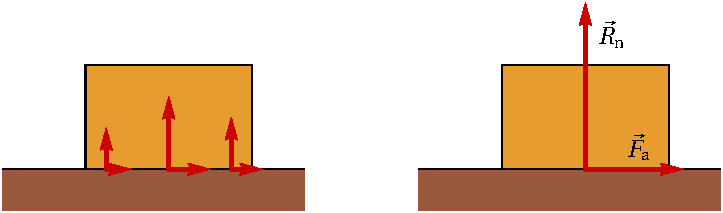
\includegraphics{normal_e_atrito.pdf}
\caption[Reação normal e força de atrito]{Reação normal $R_\mathrm{n}$
e força de atrito $\vec{F}_\mathrm{a}$ sobre um bloco na superfície
de uma mesa.}
\label{fig:contacto}
\end{figure}

\subsection{Atrito estático}
Quando não existe movimento relativo entre as duas superfícies em
contacto, a força de atrito designa-se de atrito estático. A força de
atrito estático pode ser nula, ou pode estar orientada em qualquer dos
dois sentidos na direção tangente às superfícies em contacto.

No exemplo do cavalo e o bloco (figura~\ref{fig:cavalo} na
página~\pageref{fig:cavalo}) as forças de atrito nas ferraduras do
cavalo são de atrito estático e apontam no sentido em que o cavalo
está a andar.

\subsection{Atrito cinético}
Quando as duas superfícies em contacto deslizam entre si, a força de
atrito designa-se de atrito cinético. No exemplo do cavalo e o bloco
(figura~\ref{fig:cavalo}) a força de atrito que atua no bloco é atrito
cinético e aponta no sentido oposto ao movimento.
A força de atrito cinético é sempre oposta ao movimento e tem módulo
constante, diretamente proporcional à reação normal.

O texto para este exemplo de relatório em \LaTeX\ foi extraído de
\url{https://villate.org/dinamica/index.html}.

\begin{thebibliography}{9}
\bibitem{Newton}
  Newton, Isaac (1687). \emph{Princípios Matemáticos da Filosofia
    Natural}. Tradução de J. R. Rodrigues, 2010, Lisboa, Portugal:
  Fundação Calouste Gulbenkian.
\bibitem{French}
  French, Anthony P. (1971). \emph{Newtonian Mechanics}. New York, NY,
  USA: W. W. Norton \& Company.
\end{thebibliography}
\end{document}
